%%%%%%%%%%%%%%%%%%%%%%%%%%%%%%%%%%%%%%%%%%%%%%%%%%%%%%%%%%%%%%%

%
% Welcome to Overleaf --- just edit your LaTeX on the left,
% and we'll compile it for you on the right. If you give 
% someone the link to this page, they can edit at the same
% time. See the help menu above for more info. Enjoy!
%
%%%%%%%%%%%%%%%%%%%%%%%%%%%%%%%%%%%%%%%%%%%%%%%%%%%%%%%%%%%%%%%

%  My thanks to Dana Ernst of Northern Arizona University for sharing 
%    his template with me. This is largely his work.
% --------------------------------------------------------------
% This is all preamble stuff that you don't have to worry about.
% Head down to where it says "Start here"
% --------------------------------------------------------------
 
\documentclass[12pt]{article}
 
\usepackage[margin=1in]{geometry} 
\usepackage{amsmath,amsthm,amssymb}
\usepackage{graphicx}
\usepackage{hyperref}
\usepackage{float}
\usepackage[table,x11names]{xcolor}
\usepackage[lined, linesnumbered]{algorithm2e}
\usepackage{tikz}
\makeatletter
\newenvironment{btHighlight}[1][]
{\begingroup\tikzset{bt@Highlight@par/.style={#1}}\begin{lrbox}{\@tempboxa}}
{\end{lrbox}\bt@HL@box[bt@Highlight@par]{\@tempboxa}\endgroup}

\newcommand\btHL[1][]{%
  \begin{btHighlight}[#1]\bgroup\aftergroup\bt@HL@endenv%
}
\def\bt@HL@endenv{%
  \end{btHighlight}%   
  \egroup
}
\newcommand{\bt@HL@box}[2][]{%
  \tikz[#1]{%
    \pgfpathrectangle{\pgfpoint{1pt}{0pt}}{\pgfpoint{\wd #2}{\ht #2}}%
    \pgfusepath{use as bounding box}%
    \node[anchor=base west, fill=orange!30,outer sep=0pt,inner xsep=1pt, inner ysep=0pt, rounded corners=3pt, minimum height=\ht\strutbox+1pt,#1]{\raisebox{1pt}{\strut}\strut\usebox{#2}};
  }%
}
\makeatother

\usepackage[listings,skins]{tcolorbox}
\tcbset{colback=gray!1!white,colframe=black}




\newenvironment{theorem}[2][Theorem]{\begin{trivlist}
\item[\hskip \labelsep {\bfseries #1}\hskip \labelsep {\bfseries #2.}]}{\end{trivlist}}
\newenvironment{lemma}[2][Lemma]{\begin{trivlist}
\item[\hskip \labelsep {\bfseries #1}\hskip \labelsep {\bfseries #2.}]}{\end{trivlist}}
\newenvironment{conjecture}[2][Conjecture]{\begin{trivlist}
\item[\hskip \labelsep {\bfseries #1}\hskip \labelsep {\bfseries #2.}]}{\end{trivlist}}
\newenvironment{question}[2][Question]{\begin{trivlist}
\item[\hskip \labelsep {\bfseries #1}\hskip \labelsep {\bfseries #2.}]}{\end{trivlist}}
\newenvironment{corollary}[2][Corollary]{\begin{trivlist}
\item[\hskip \labelsep {\bfseries #1}\hskip \labelsep {\bfseries #2.}]}{\end{trivlist}}
\newenvironment{definition}[2][Definition]{\begin{trivlist}
\item[\hskip \labelsep {\bfseries #1}\hskip \labelsep {\bfseries #2.}]}{\end{trivlist}}


\definecolor{commentgreen}{RGB}{176, 176, 176}
\definecolor{rowcolor}{cmyk}{0,0.87,0.68,0.32}
\definecolor{rowcolor2}{cmyk}{ 20, 0, 37, 34}

\definecolor{eminence}{RGB}{108,48,130}
\definecolor{weborange}{RGB}{255,165,0}
\definecolor{frenchplum}{RGB}{129,20,82}
\definecolor{darkgreen}{RGB}{10, 92, 10}


\definecolor{celadon}{rgb}{0.67, 0.88, 0.69}

\definecolor{mGreen}{rgb}{0,0.6,0}
\definecolor{mGray}{rgb}{0.5,0.5,0.5}
\definecolor{mPurple}{rgb}{0.58,0,0.82}
\definecolor{backgroundColour}{rgb}{0.95,0.95,0.92}

\lstdefinestyle{CStyle}{
    commentstyle=\color{mGreen},
    keywordstyle=\color{magenta},
    numberstyle=\tiny\color{mGray},
    stringstyle=\color{mPurple},
    basicstyle=\footnotesize,
    breakatwhitespace=false,         
    breaklines=true,                 
    captionpos=b,                    
    keepspaces=true,                 
    numbers=left,                    
    numbersep=5pt,                  
    showspaces=false,                
    showstringspaces=false,
    showtabs=false,                  
    tabsize=2,
    language=C,
    moredelim=**[is][{\btHL[celadon!40]}]{`}{`}
}

\lstdefinestyle{nccode}{
    numbers=none,
    stepnumber=1,
    numbersep=10pt,
    tabsize=4,
    showspaces=false,
    breaklines=true, 
    showstringspaces=false,
    moredelim=**[is][{\btHL[orange!50]}]{`}{`}
}

\begin{document}
 
% --------------------------------------------------------------
%                         Start here
% --------------------------------------------------------------
 
\title{Assignment 3: MPI Programming} % replace with an appropriate title, choose something shortish & descriptive
\author{Javier Cabrera Arteaga, Deepika Tiwari} % replace with your name, multiple authors go in alphabetical order by last name
 
\maketitle

{%
\centering
FDD3258 - Introduction to High-Performance Computing (MPI module)
\par
}
\hrule
\vspace{.2in}

\section{Exercise 1 - MPI Hello World, Get Familiar with the MPI Environment}
\begin{enumerate}
    \item Write the Hello World Code in C\\
    \begin{lstlisting}[style=CStyle]
#include <mpi.h>
#include <stdio.h>

int main(int argc, char *argv[]){

	int rank, size, i, provided;

	MPI_Init_thread(&argc, &argv, MPI_THREAD_SINGLE, &provided);

	MPI_Comm_size(MPI_COMM_WORLD, &size);
	MPI_Comm_rank(MPI_COMM_WORLD, &rank);

	printf("My rank %d of %d\n", rank, size);

	MPI_Finalize();
	return 0;
}
	\end{lstlisting}
	
\textit{Sample output:}
\begin{lstlisting}
My rank 0 of 5
My rank 1 of 5
My rank 2 of 5
My rank 3 of 5
My rank 4 of 5
\end{lstlisting}
	
	\item Answer the following questions:
	\begin{itemize}
	    \item How do you compile it, which compiler and flags have you used if any?\\
	    The above code is compiled on Beskow with \texttt{cc hello.c -o hello.out}
	    \item How do you run the MPI code on Beskow?\\
	    To run the compiled code on Beskow, we first ask for allocation with \texttt{salloc --nodes=1 -t 01:00:00 -A edu20.FDD3258} and then run with \texttt{srun -n 5 ./hello.out}
	    \item How do you change the number of MPI processes?\\
	    The number of MPI processes can be set via the \texttt{n} flag specified with \texttt{srun}. For instance, \texttt{srun -n 5 ./hello.out} will spawn 5 processes, and \texttt{srun -n 10 ./hello.out} will spawn 10.
	    \item Which functions do you use for retrieving the rank of an MPI process and the total number of processes?\\
	    \texttt{MPI\_Comm\_rank(MPI\_COMM\_WORLD, \&rank);} is the function call that retrieves the rank (or identifier) of the current MPI process and saves it into the integer \texttt{rank} variable. \texttt{MPI\_Comm\_size(MPI\_COMM\_WORLD, \&size);} retrieves the total number of MPI processes and saves the value in the integer \texttt{size} variable. Both of these values are obtained from the default MPI communicator, \texttt{MPI\_COMM\_WORLD}.
	    \item What are the names of the most used MPI implementations?\\
	    The most popular implementations compliant with the MPI standard are MPICH and OpenMPI.
	\end{itemize}
\end{enumerate}

\section{Exercise 2 - Calculate PI with MPI}
\subsection{MPI Blocking Communication \& Linear Reduction Algorithm}
\begin{enumerate}
    \item Implement the code using a linear algorithm with MPI Send/Recv\\
    We implement blocking communication through \texttt{MPI\_Send()} and \texttt{MPI\_Recv()} to calculate the value of PI with MPI. The code is available in the solution repository at the path \textit{HPC\_mpi/pi/pi\_blocking.c}.
    \item Measure the performance of the code (execution time) for 8, 16, 32,  64, 128 MPI processes and plot it
    \begin{figure}[H]
        \centering
        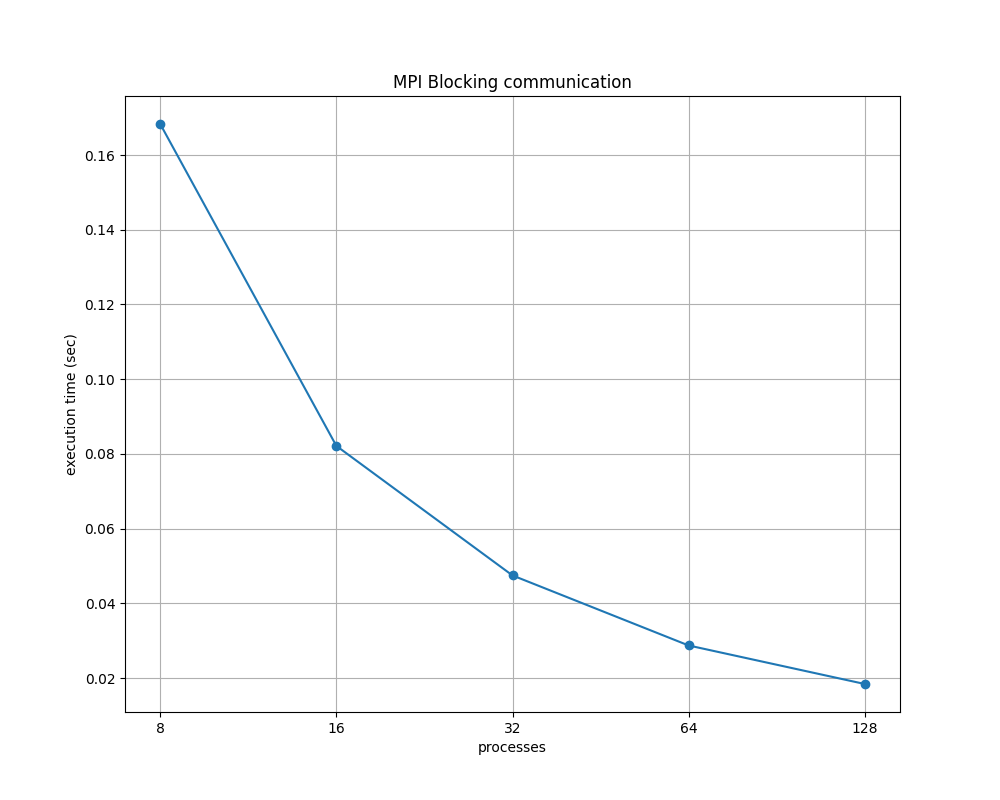
\includegraphics[width=0.8\textwidth]{graph-pi-blocking.png}
        \caption{MPI Blocking Communication between 8 to 128 processes}
        \label{fig:blocking}
    \end{figure}
% deepikat@beskow-login2:/cfs/klemming/scratch/d/deepikat/pi> srun -n 5 ./pi_blocking.out 
% pi: 3.141475
% Execution Time: 0.181464
% deepikat@beskow-login2:/cfs/klemming/scratch/d/deepikat/pi> srun -n 8 ./pi_blocking.out 
% pi: 3.141570
% Execution Time: 0.168313
% deepikat@beskow-login2:/cfs/klemming/scratch/d/deepikat/pi> srun -n 16 ./pi_blocking.out 
% pi: 3.141408
% Execution Time: 0.082145
% deepikat@beskow-login2:/cfs/klemming/scratch/d/deepikat/pi> srun -n 32 ./pi_blocking.out 
% pi: 3.141634
% Execution Time: 0.047470
% deepikat@beskow-login2:/cfs/klemming/scratch/d/deepikat/pi> srun -n 64 ./pi_blocking.out 
% pi: 3.141428
% Execution Time: 0.028720
% deepikat@beskow-login2:/cfs/klemming/scratch/d/deepikat/pi> srun -n 128 ./pi_blocking.out 
% pi: 3.141850
% Execution Time: 0.018408


    \item Answer the following questions:
    \begin{itemize}
        \item Why are \texttt{MPI\_Send()} and \texttt{MPI\_Recv()} called "blocking" communication?\\
         \texttt{MPI\_Send()} and \texttt{MPI\_Recv()} do not return before the MPI buffer is safe for reuse, i.e., they "block" further execution of the program till communication completes.
        \item What is the MPI function for timing?\\
        \texttt{MPI\_Wtime()} enables the measurement of wall time with MPI.
    \end{itemize}
\end{enumerate}

\subsection{MPI Blocking Communication \& Binary Tree Reduction Communication Algorithm}

\subsection{MPI Non-Blocking Communication \& Linear Reduction Algorithm}

\begin{enumerate}
	\item Implement the code using non-blocking communication.
	
	The code is available in \textit{HPC\_mpi/pi/pi\_non\_blocking.c}.
	\item  Measure the performance of the code (execution time) for 8, 16, 32,  64, 128 MPI processes and plot it
	Answer the following questions:
	\begin{enumerate}
		\item What are the MPI functions for non-blocking communication? 
		
		The functions for non-blocking communication are 
		
		\texttt{MPI
		\_Irecv()} Register a callback buffer to add the result without waiting blocking the execution


		\texttt{MPI\_Waitall()} Wait for all made calls registered before by \texttt{MPI
		\_Irecv()}

		The previous mentioned method for blocking calls can be used as well with these non-blocking method. This can be appreciated in \url{https://github.com/Jacarte/HPC_mpi/blob/ca767b5958557a4f4b1d8cfb79d6e91e8662fed7/pi/pi_non_blocking.c#L66}

		

		\item What does the "I" in front of function name stand for in non-blocking communication?
		
		The 'I' in MPI non-blocking communication methods stands for immediate.

		\item How the performance of non-blocking communication compares to the performance of blocking communication. e.g. performance results in 2.1?
  
% javierca@beskow-login2:/cfs/klemming/scratch/j/javierca/HPC_MPI/HPC_mpi/pi> srun -n 5 non_blocking.out 
% pi: 3.141114
% Execution Time: 0.111884
% javierca@beskow-login2:/cfs/klemming/scratch/j/javierca/HPC_MPI/HPC_mpi/pi> srun -n 8 non_blocking.out 
% pi: 3.141549
% Execution Time: 0.077699
% javierca@beskow-login2:/cfs/klemming/scratch/j/javierca/HPC_MPI/HPC_mpi/pi> srun -n 16 non_blocking.out 
% pi: 3.141375
% Execution Time: 0.044840
% javierca@beskow-login2:/cfs/klemming/scratch/j/javierca/HPC_MPI/HPC_mpi/pi> srun -n 32 non_blocking.out 
% pi: 3.142038
% Execution Time: 0.022413
% javierca@beskow-login2:/cfs/klemming/scratch/j/javierca/HPC_MPI/HPC_mpi/pi> srun -n 64 non_blocking.out 
% pi: 3.141475
% Execution Time: 0.012153
% javierca@beskow-login2:/cfs/klemming/scratch/j/javierca/HPC_MPI/HPC_mpi/pi> srun -n 128 non_blocking.out 
% pi: 3.142132
% Execution Time: 0.009045
% javierca@beskow-login2:/cfs/klemming/scratch/j/javierca/HPC_MPI/HPC_mpi/pi> 
\begin{figure}[H]
  \centering
  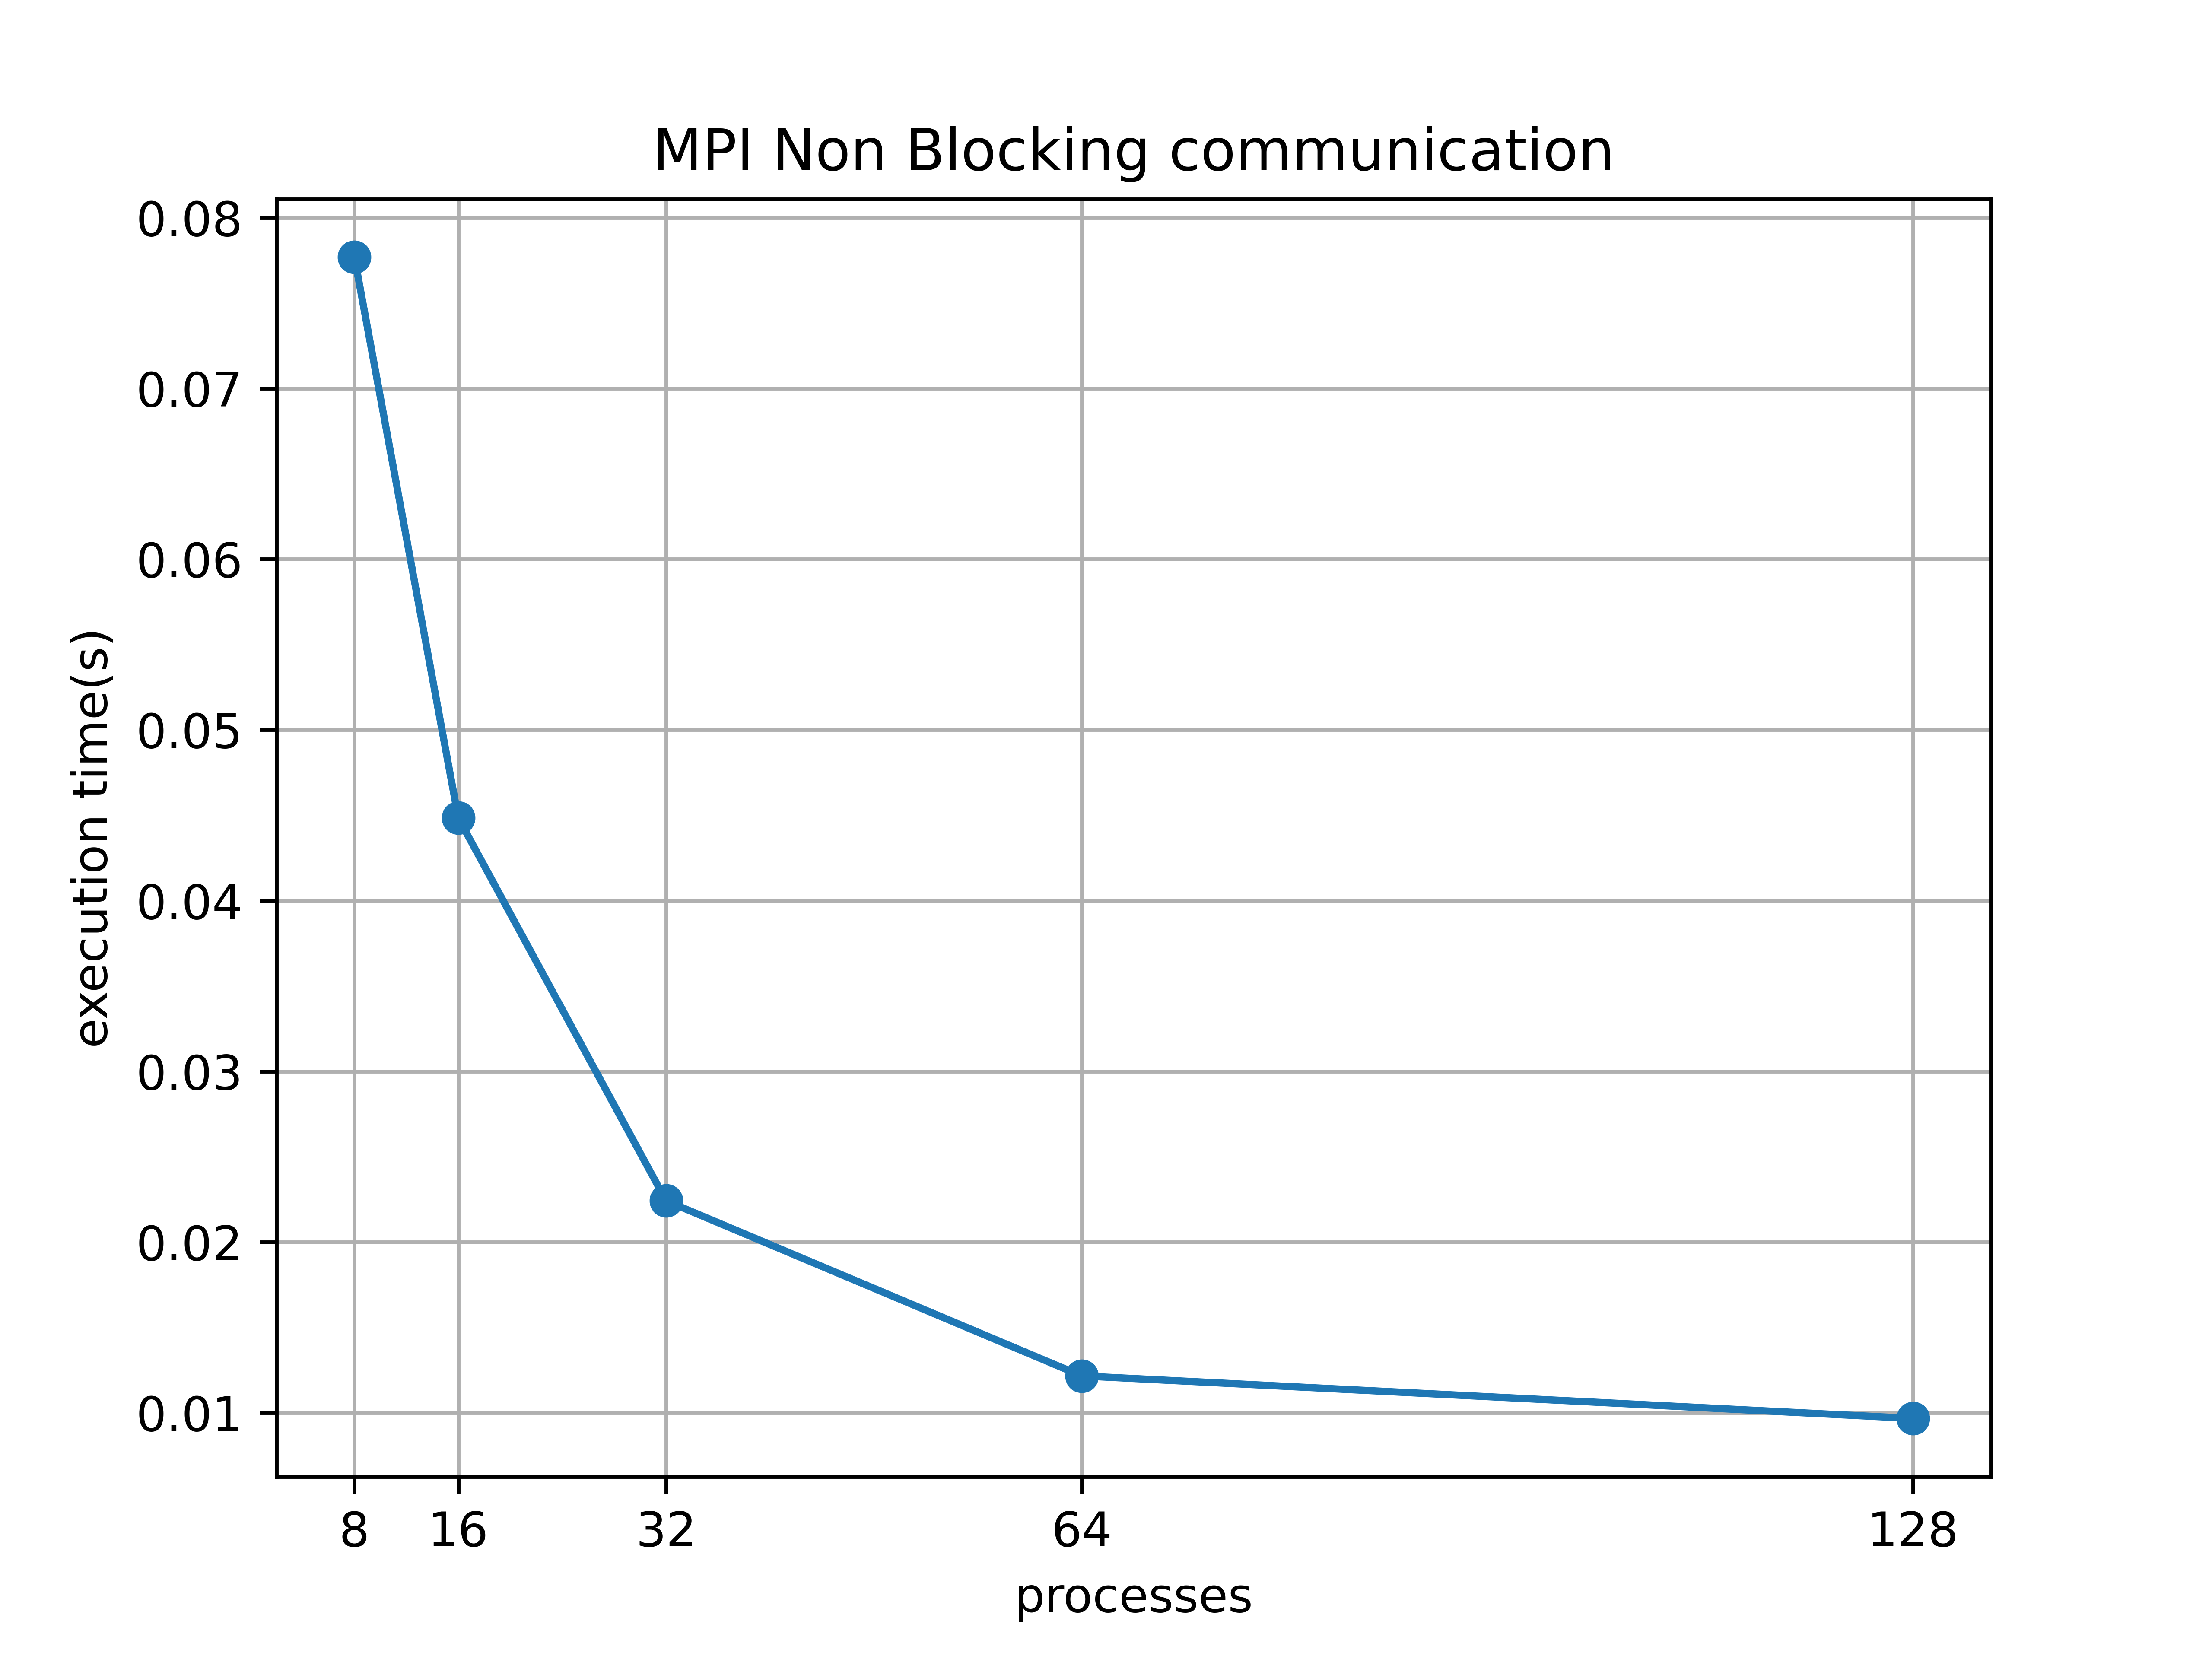
\includegraphics[width=0.8\textwidth]{graph-pi-non-blocking.png}
  \caption{MPI Non Blocking Communication between 8 to 128 processes}
  \label{fig:blocking}
\end{figure}

The non-blocking approach performs better since the manager process (rank 0) does not wait for the others to calculate its part.

  \end{enumerate}
	
\end{enumerate}


\subsection{MPI Collective MPI\_Gather}

\begin{enumerate}
  
  \item Implement the code using non-blocking communication.
    
  The code is available in \textit{HPC\_mpi/pi/pi\_gather.c}.
  \item  Measure the performance of the code (execution time) for 8, 16, 32,  64, 128 MPI processes and plot it
   
  \begin{figure}[H]
    \centering
    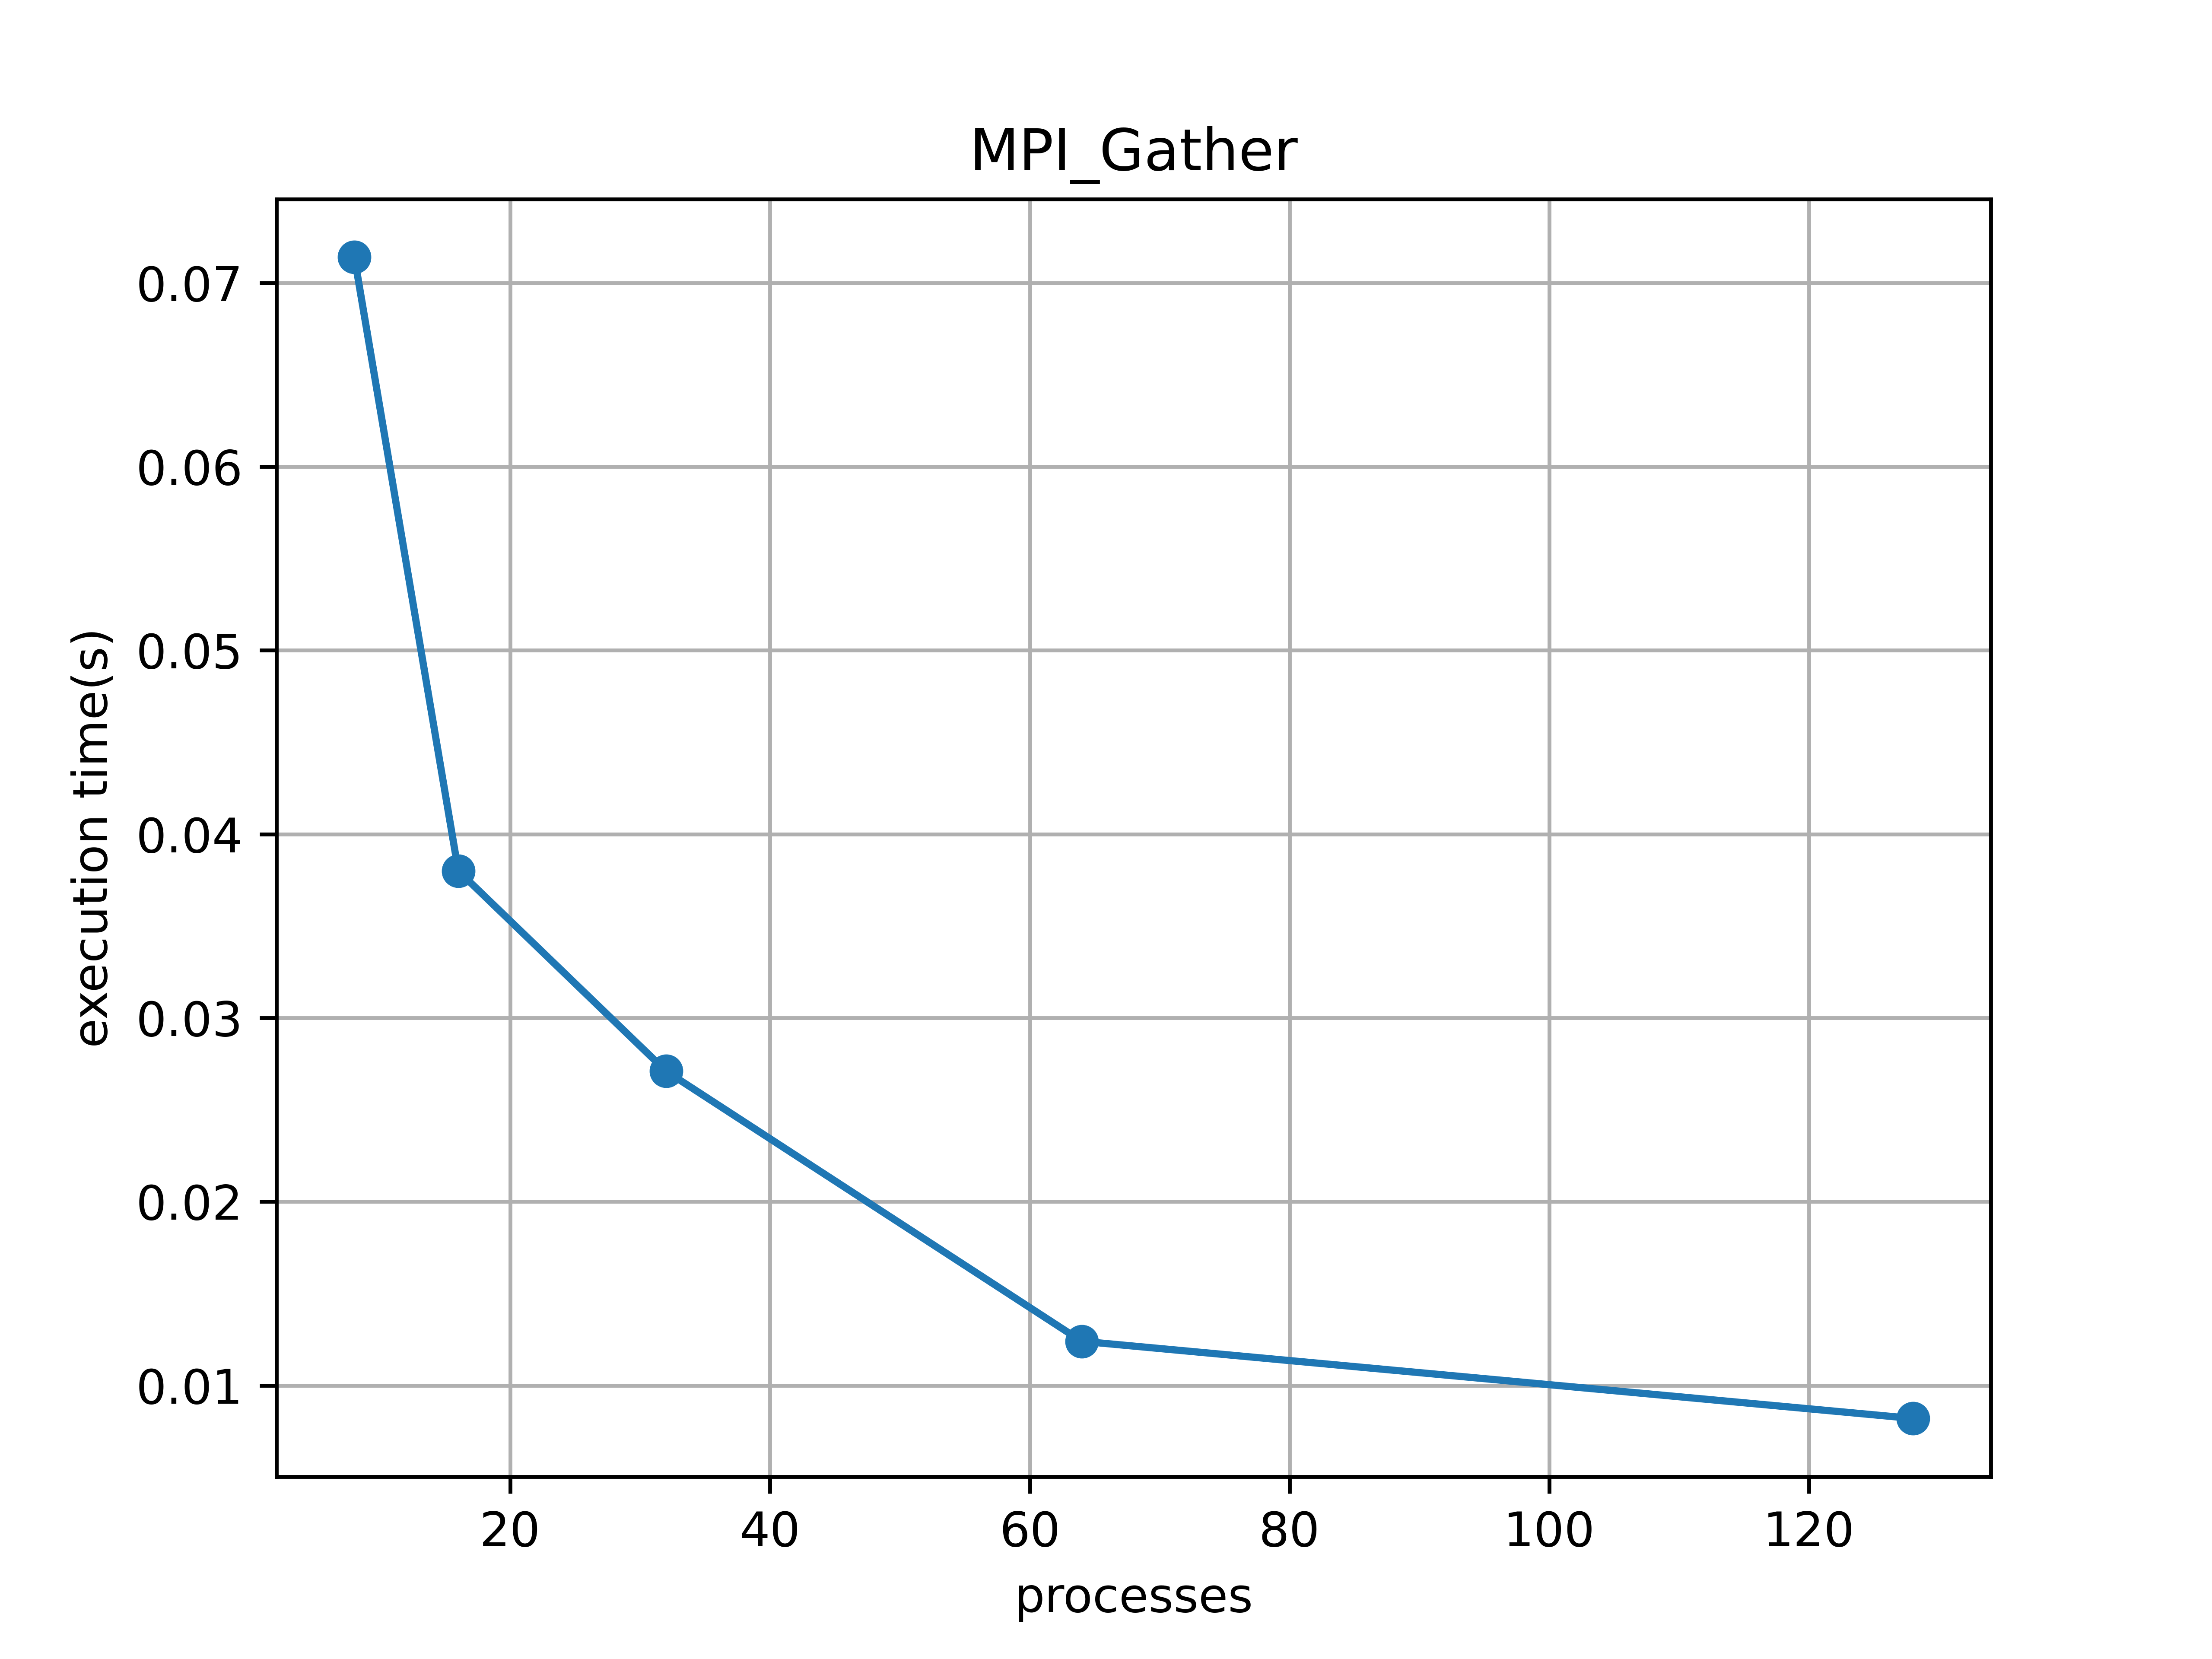
\includegraphics[width=0.8\textwidth]{graph-pi-mpi-gather.png}
    \caption{MPI\_Gather 8 to 128 processes}
    \label{fig:blocking}
  \end{figure}
\end{enumerate}

% javierca@beskow-login2:/cfs/klemming/scratch/j/% javierca/HPC_MPI/HPC_mpi/pi> srun -n 8 gather.out 
% pi: 3.141302
% Execution Time: 0.071430
% javierca@beskow-login2:/cfs/klemming/scratch/j/% javierca/HPC_MPI/HPC_mpi/pi> srun -n 16 gather.out 
% pi: 3.140568
% Execution Time: 0.038054
% javierca@beskow-login2:/cfs/klemming/scratch/j/% javierca/HPC_MPI/HPC_mpi/pi> srun -n 32 gather.out 
% pi: 3.141721
% Execution Time: 0.027142
% javierca@beskow-login2:/cfs/klemming/scratch/j/% javierca/HPC_MPI/HPC_mpi/pi> srun -n 64 gather.out 
% pi: 3.141775
% Execution Time: 0.012407
% javierca@beskow-login2:/cfs/klemming/scratch/j/% javierca/HPC_MPI/HPC_mpi/pi> srun -n 128 gather.% out 
% pi: 3.141996
% Execution Time: 0.008289
% javierca@beskow-login2:/cfs/klemming/scratch/j/% javierca/HPC_MPI/HPC_mpi/pi> 

\subsection{MPI Collective MPI\_Reduce}

\begin{enumerate}
  
  \item Implement the code using non-blocking communication.
    
  The code is available in \textit{HPC\_mpi/pi/pi\_collective.c}.
  \item  Measure the performance of the code (execution time) for 8, 16, 32,  64, 128 MPI processes and plot it
   
  \begin{figure}[H]
    \centering
    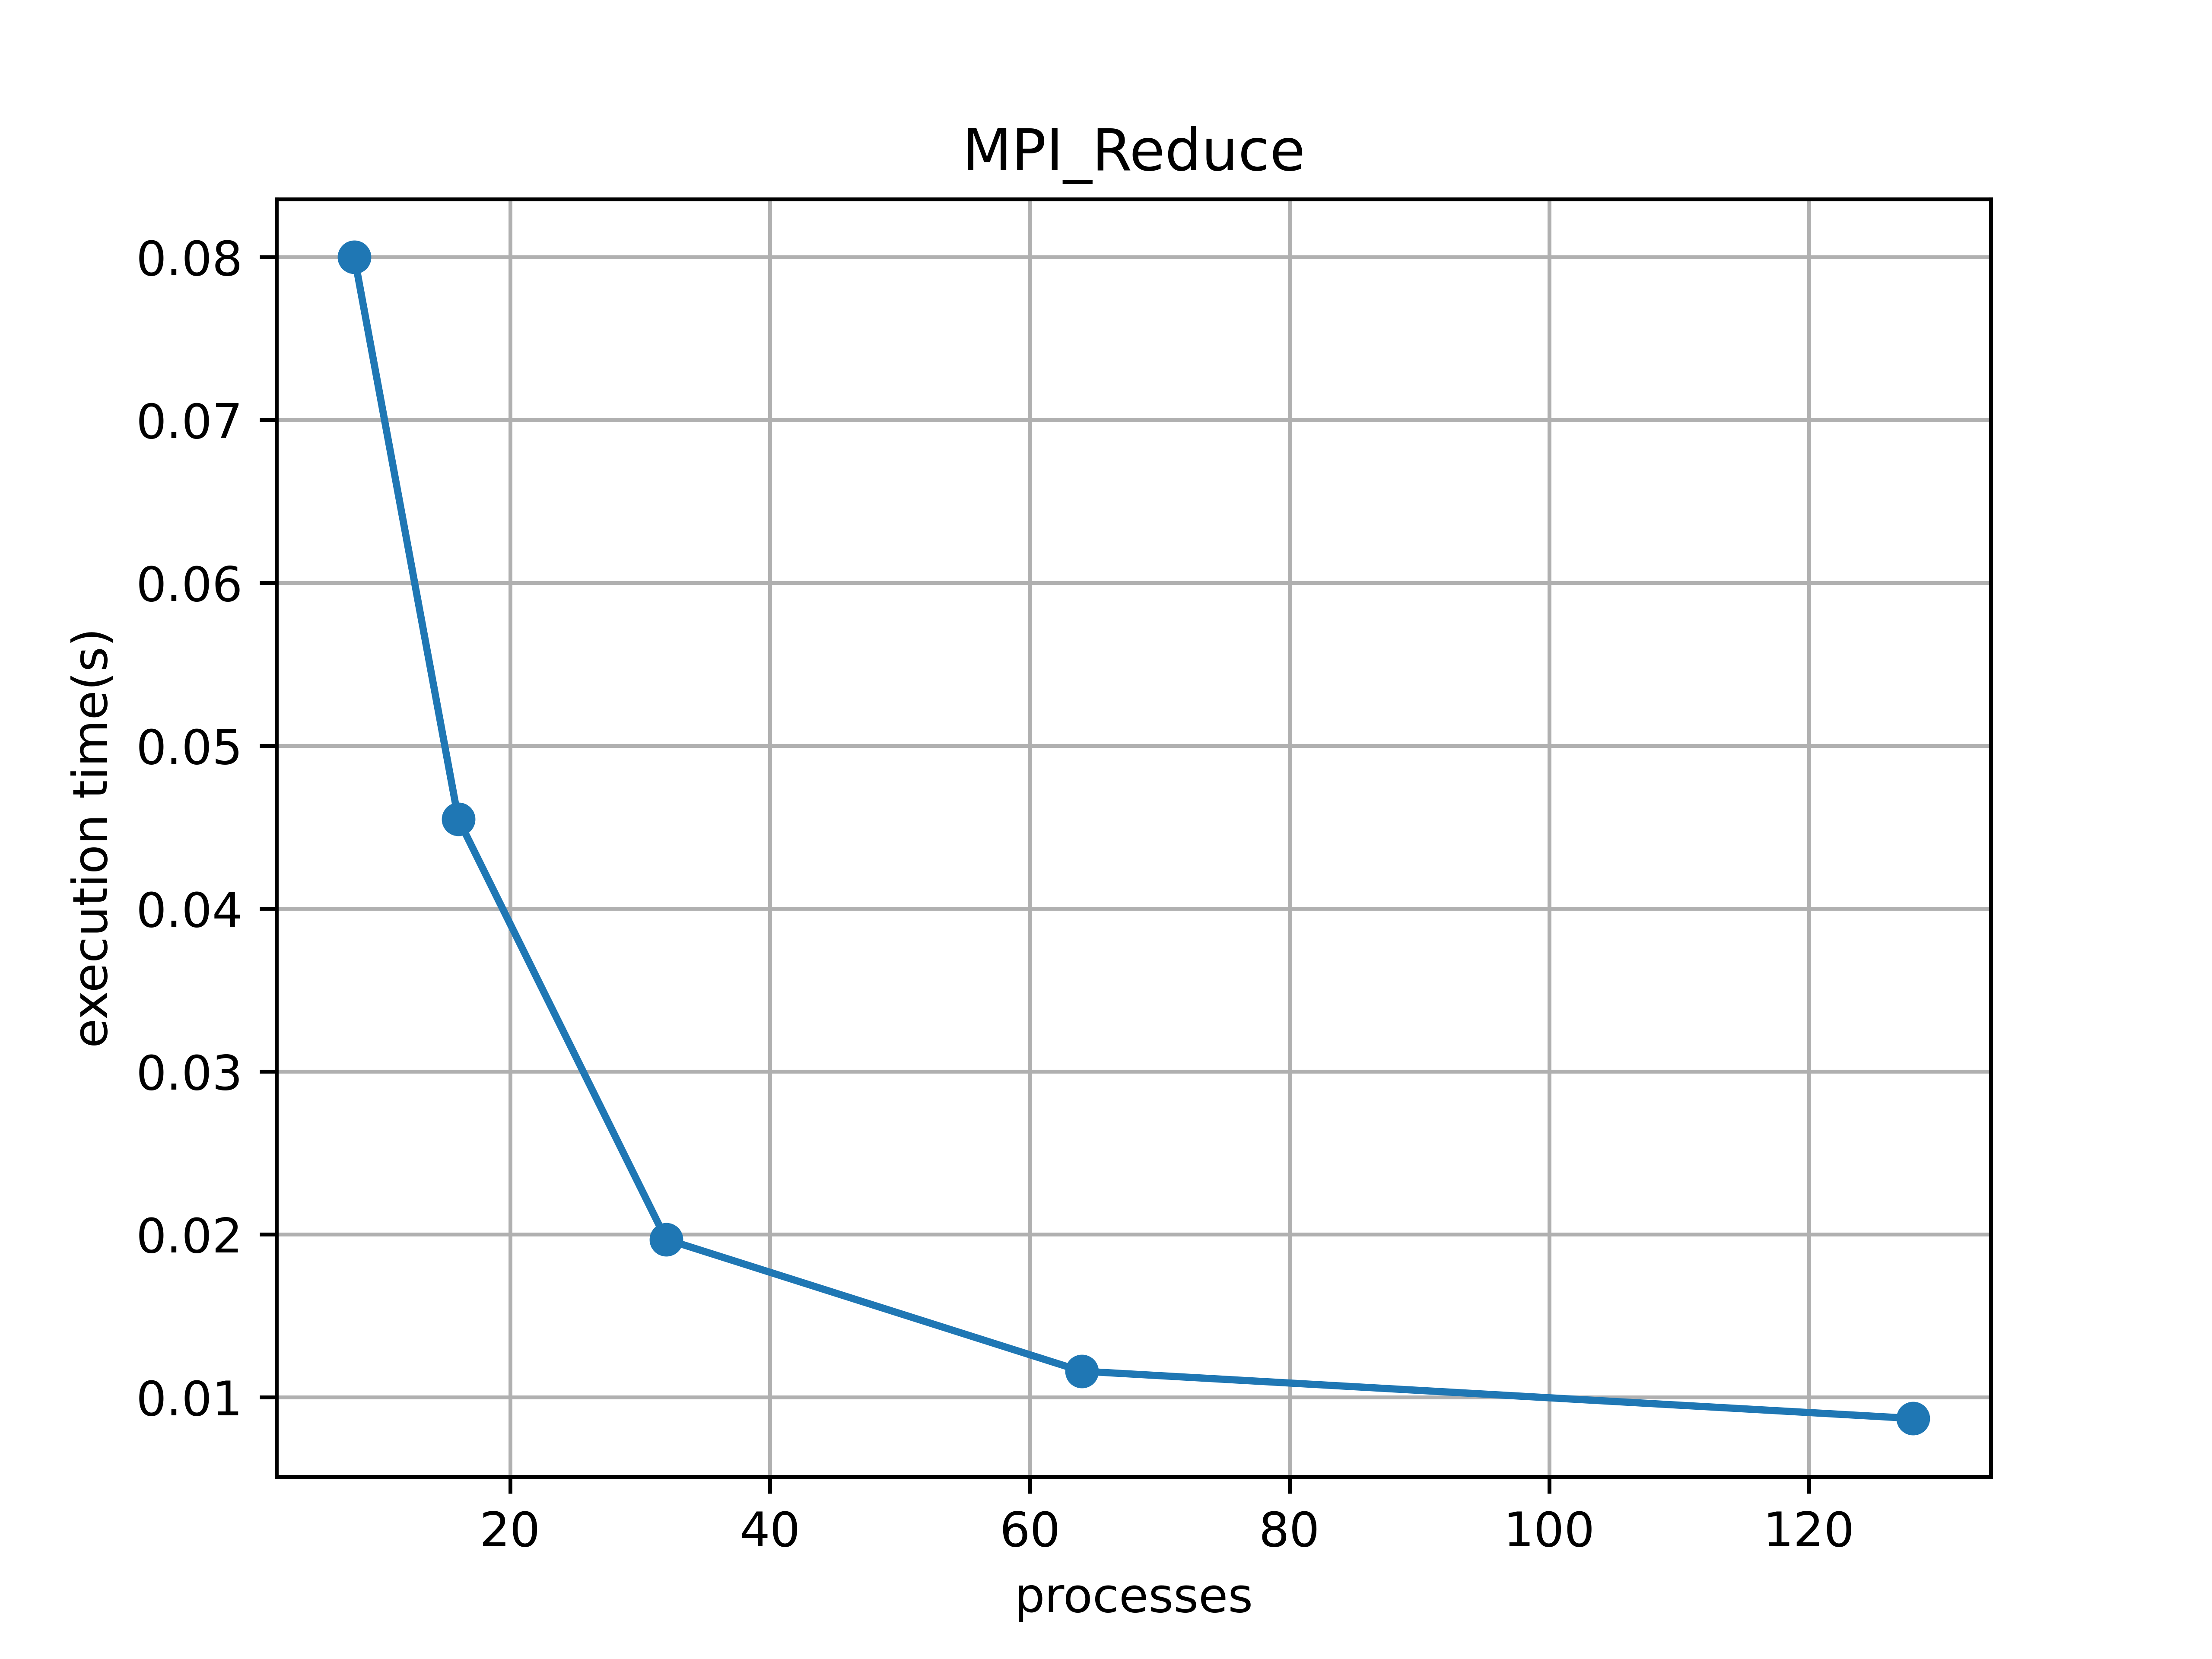
\includegraphics[width=0.8\textwidth]{graph-pi-mpi-reduce.png}
    \caption{MPI\_Reduce 8 to 128 processes}
    \label{fig:blocking}
  \end{figure}
\end{enumerate}
% javierca@beskow-login2:/cfs/klemming/scratch/j/% javierca/HPC_MPI/HPC_mpi/pi> srun -n 8 collective.% out 
% pi: 3.141894
% Execution Time: 0.080002
% javierca@beskow-login2:/cfs/klemming/scratch/j/% javierca/HPC_MPI/HPC_mpi/pi> srun -n 16 collective.% out 
% pi: 3.141840
% Execution Time: 0.045499
% javierca@beskow-login2:/cfs/klemming/scratch/j/% javierca/HPC_MPI/HPC_mpi/pi> srun -n 32 collective.% out 
% pi: 3.141454
% Execution Time: 0.019708
% javierca@beskow-login2:/cfs/klemming/scratch/j/% javierca/HPC_MPI/HPC_mpi/pi> srun -n 64 collective.% out 
% pi: 3.141425
% Execution Time: 0.011591
% javierca@beskow-login2:/cfs/klemming/scratch/j/% javierca/HPC_MPI/HPC_mpi/pi> srun -n 128 % collective.out 
% pi: 3.141079
% Execution Time: 0.008663


\begin{figure}[H]
  \centering
  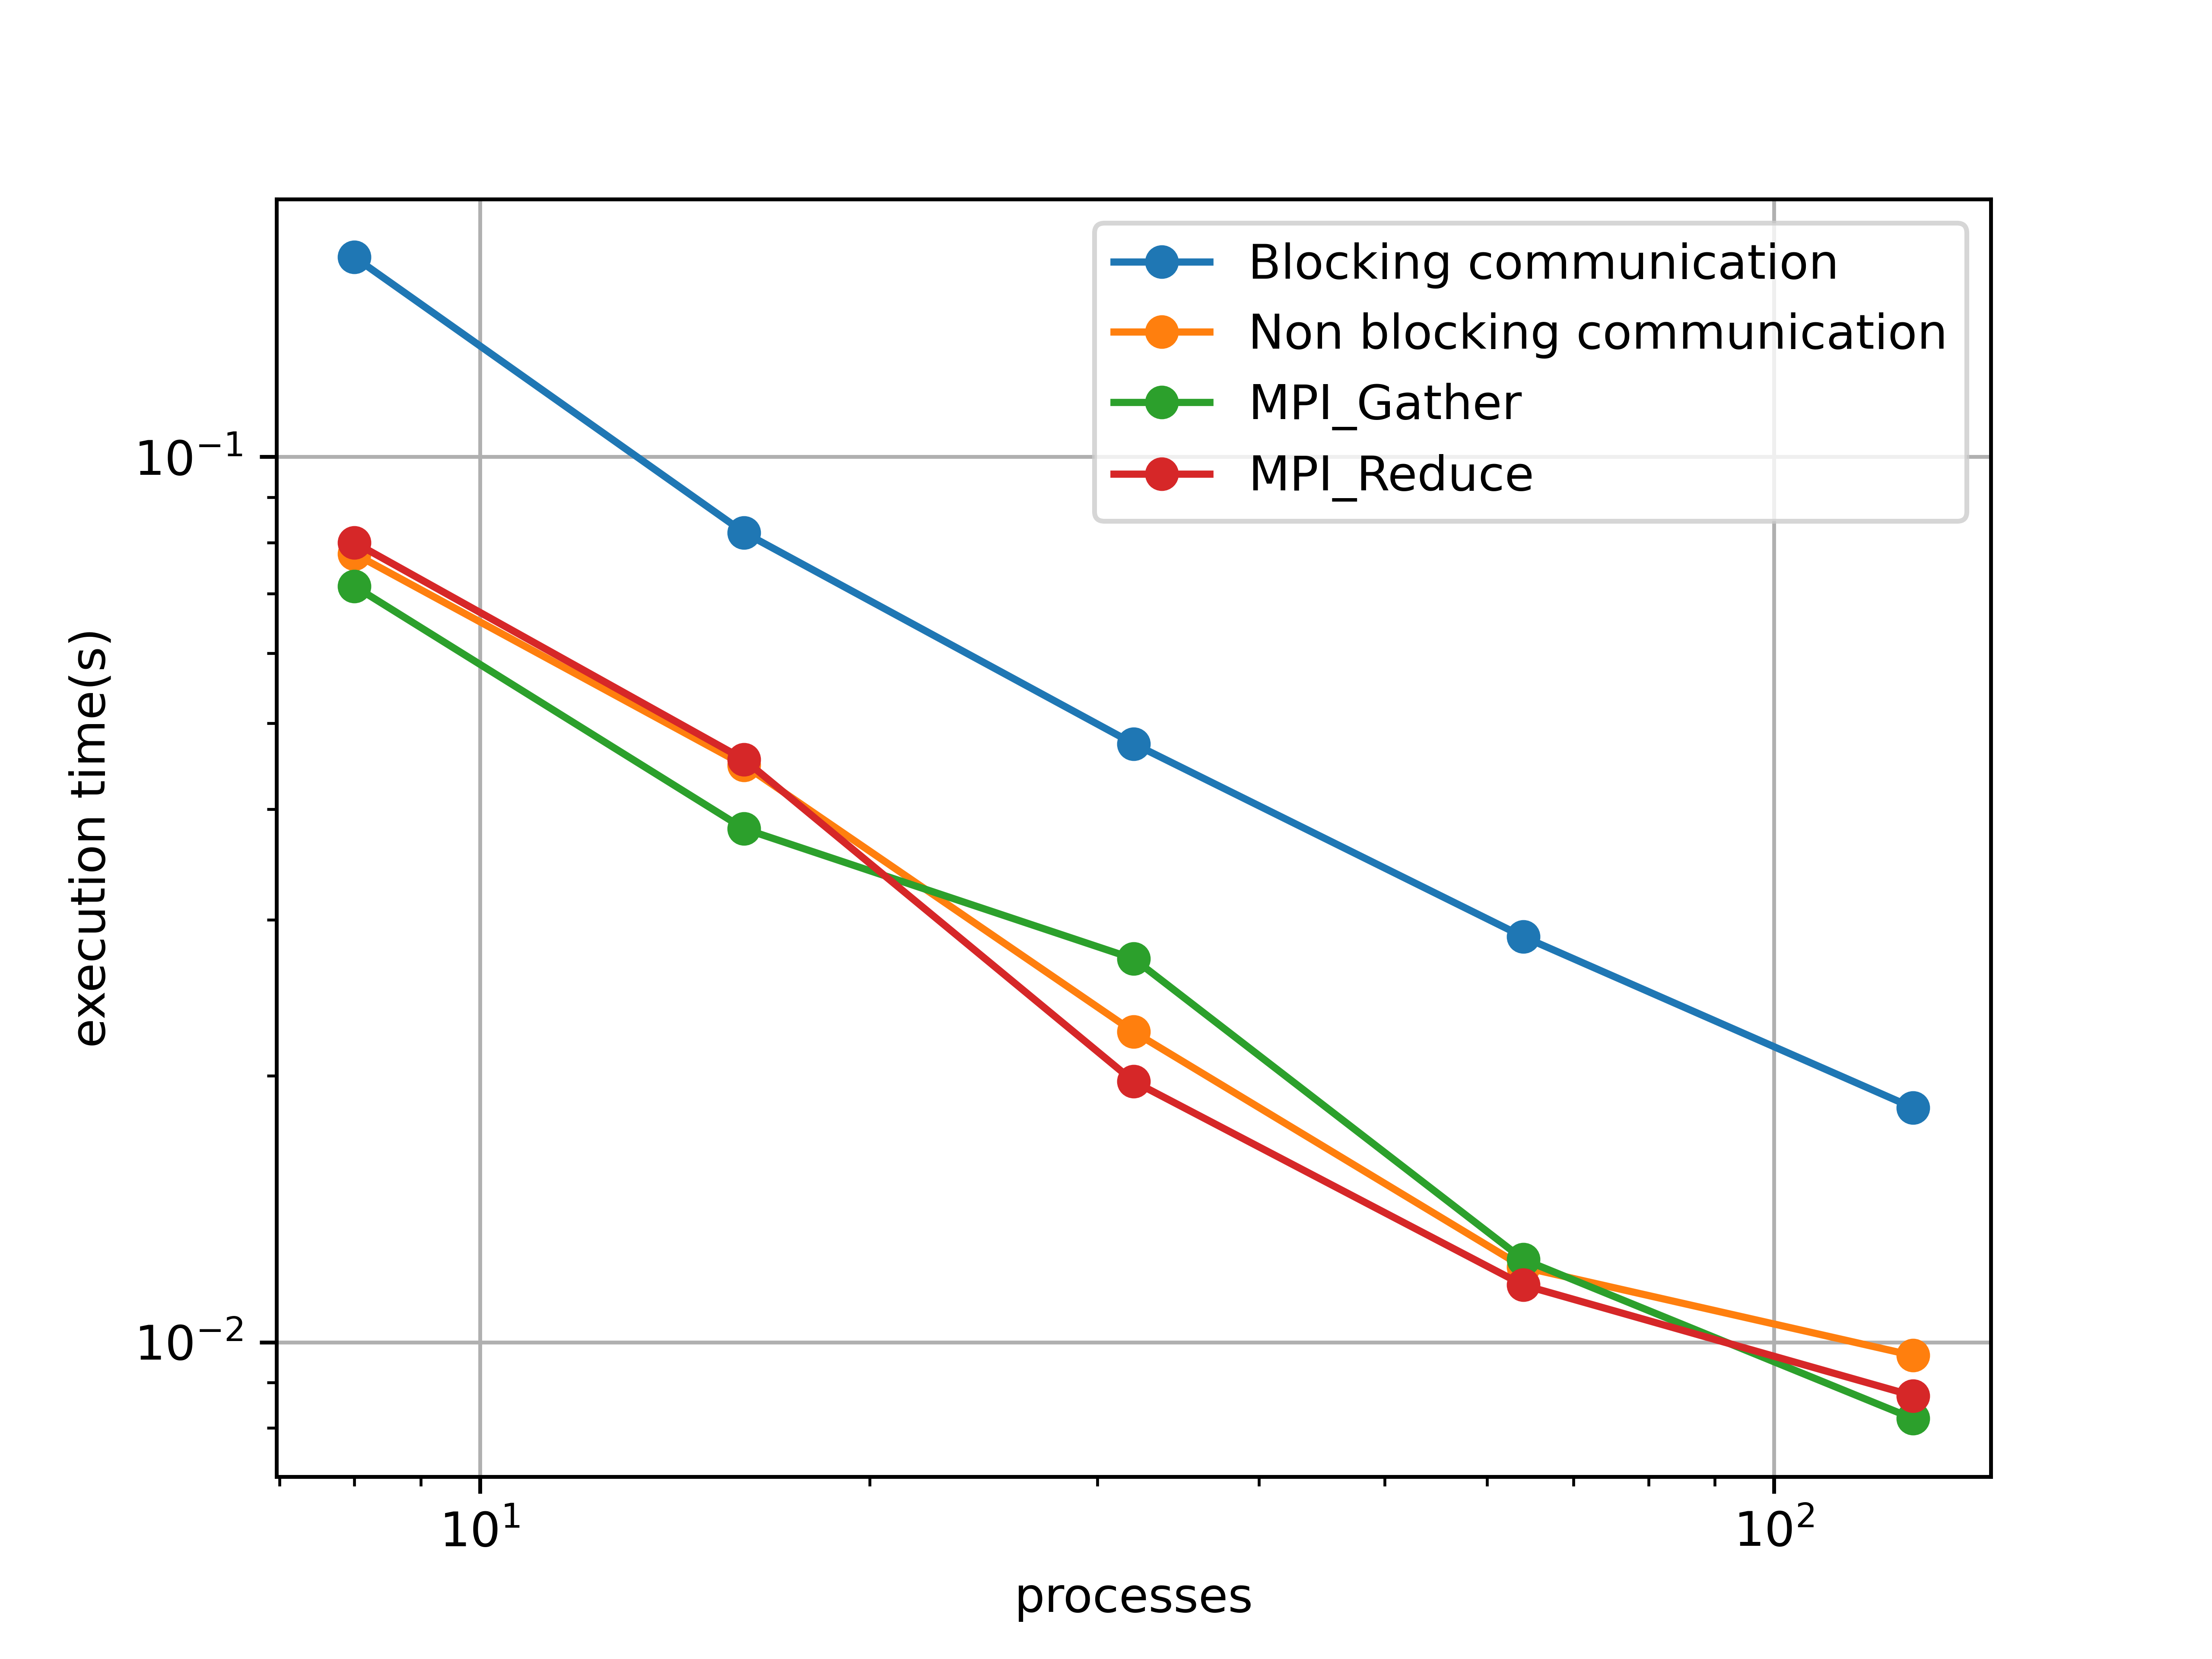
\includegraphics[width=0.8\textwidth]{all.png}
  \caption{PI calculation with all approaches.}
  \label{fig:blocking}
\end{figure}

\section{Exercise 3}
Run the ping-pong code and calculate the bandwidth and latency for
\begin{enumerate}
    \item intra-node communication (2 processes on the same node)
    \item inter-node communication (2 processes on different nodes)
\end{enumerate}
Questions:
\begin{enumerate}
    \item Run the ping-pong benchmark for 1) and 2).
    \begin{itemize}
        \item To run 2 processes on the same node, we use the following commands on Beskow:\\
        \texttt{salloc --nodes=1 -t 00:05:00 -A edu20.FDD3258 -C Haswell}\\
        \texttt{srun -n 2 ./ping\_pong.out}

%          8	    0.000000608
%         16	    0.000000653
%         32	    0.000000682
%         64	    0.000000734
%        128	    0.000000770
%        256	    0.000000751
%        512	    0.000000815
%       1024	    0.000000978
%       2048	    0.000001161
%       4096	    0.000001707
%       8192	    0.000003898
%      16384	    0.000004125
%      32768	    0.000007594
%      65536	    0.000011530
%     131072	    0.000024257
%     262144	    0.000045474
%     524288	    0.000088394
%    1048576	    0.000173810
%    2097152	    0.000345354
%    4194304	    0.000689859
%    8388608	    0.001377771
%   16777216	    0.002741075
%   33554432	    0.005612578
%   67108864	    0.011531770
%  134217728	    0.023308010
%  268435456	    0.046876423
%  536870912	    0.094284530
% 1073741824	    0.193143849

        \item To run 2 processes on different nodes, we use the following commands on Beskow:\\
        \texttt{salloc --nodes=2 -t 01:00:00 -A edu20.FDD3258 -C Haswell}\\
        \texttt{srun -n 2 --ntasks-per-node=1 ./ping\_pong.out}

%          8	    0.000001717
%         16	    0.000001941
%         32	    0.000001702
%         64	    0.000001564
%        128	    0.000001600
%        256	    0.000001712
%        512	    0.000001829
%       1024	    0.000001943
%       2048	    0.000002546
%       4096	    0.000003426
%       8192	    0.000006628
%      16384	    0.000006628
%      32768	    0.000008008
%      65536	    0.000013492
%     131072	    0.000021279
%     262144	    0.000032403
%     524288	    0.000058684
%    1048576	    0.000116324
%    2097152	    0.000225928
%    4194304	    0.000471337
%    8388608	    0.000999577
%   16777216	    0.002077246
%   33554432	    0.004228852
%   67108864	    0.008591294
%  134217728	    0.017421808
%  268435456	    0.034961929
%  536870912	    0.071018376
% 1073741824	    0.143390267

    \end{itemize}

    \item Plot ping-pong time in function of the message size for 1) and 2).

    \begin{figure}[H]
    \centering
    \includegraphics[width=0.8\textwidth]{graph-ping-pong.png}
    \caption{Ping-pong for intra- and inter-node communication on Beskow}
    \label{fig:blocking}
  \end{figure}

    \item By best fit (using Matlab, Python, or similar), calculate the bandwidth and latency for 1) and 2).
    \item Answer the following question
    \begin{itemize}
        \item For case 2), how do the obtained values of bandwidth and latency compare to the nominal Beskow network bandwidth and latency. What are the differences and what could be the explanation of the differences if any?
    \end{itemize}
\end{enumerate}

\end{document}

